\ifdefined\COMPLETE
\else
    \input{./preambule-sacha-utf8.ltx}
    
\frenchbsetup{StandardLists=true} % à inclure si on utilise \usepackage[french]{babel}
\usepackage{enumitem}   

\usepackage{diagbox}
\frenchbsetup{StandardItemLabels=true, CompactItemize=false, ReduceListSpacing=true}

\usepackage{pdflscape}

\textwidth=21cm			
\textheight=24.5cm

    \begin{document}
\fi

\begin{landscape}


\newcommand{\case}[2]{\parbox{#1}{\footnotesize\begin{center}% Déterminer 
#2\end{center}}}

\setbox1=\hbox{{\color{blue} % Garder les doubles accolades sinon bleu se propage
\begin{tikzpicture}
   \tkzTabInit%
   [lgt = 1.5, espcl = .8, deltacl = .3]%
   {$x$ / 1 ,$x$/1, $ax -x_1$ / 1,  $ax -x_2$ / 1, p/1}{$-\infty$, $x_1$, $x_2$,$+\infty$}
   \tkzTabLine{, +,t,+,t,+, }
   \tkzTabLine{, -,z,+,t,+, }
   \tkzTabLine{, -,t,-,z,+, }
   \tkzTabLine{, +,z,-,z,+, }
\end{tikzpicture}}
}

\setbox2=\hbox{{\color{blue}
\begin{tikzpicture}
   \tkzTabInit%
      [lgt = 1.5, espcl = .8, deltacl = .3]%
      {$x$ /1,%
           $f(x)$ / 1.5}%
           {$-\infty$, $\alpha$, $+\infty$}
   \tkzTabVar{+/ , -/ $\beta$, +/ }
\end{tikzpicture}}
}

\setbox3=\hbox{{\color{blue}
\begin{tikzpicture}
   \tkzTabInit%
      [lgt = 1.5, espcl = .8, deltacl = .3]%
      {$x$ /1,%
           $f(x)$ / 1.5}%
           {$-\infty$, $\alpha$, $+\infty$}
   \tkzTabVar{-/ , +/ $\beta$, -/ }
\end{tikzpicture}}
}

\pagestyle{empty}

{\vspace*{-2cm}
\centerline{\color{red} \huge \bf Utilisation des trois formes du trinôme} 
\bigskip 
\centerline{ \begin{tabular}{|l|c|c|c|c|c|c|c|}
\hline %-----------------------------------------------
 \diagbox[width=25mm]
      {\\Forme \\ utilisée}{\\But} 
      & \case{15mm} { l'équation $f(x)=0$   }           % 2 
           &  \case{35mm} {les variations}                  % 3 
              &  \case{40mm}  { le signe du trinôme }               % 4  
                  & \case{15mm}{le sommet de la parabole}   % 5
                      &  \case{20mm}{les racines }                                          %6 
                         &  \case{15mm}{les solutions de $ f(x) \geqslant 0$  }  %7 
                           &  \case{25mm}{les images\\et les antécédents\\d'un point } %8 
      \\ % Résoudre l'équation $f(x)=0$ 
\hline %-----------------------------------------------    
% 1 & 2   & 3 & 4 & 5 & 6 & 7 & 8 
 \case {20mm}{Forme développée $ax^2 +bx +c $} 
      & \case {15mm}{\color{blue} Voir fiche associée} &  &   &  % 3 -- 5 
          & \case {20mm}{\color{blue} Les solutions de $f(x)=0$ sont les racines}   &  % 7 
              & \case {25mm}{\color{blue} On remplace $x$\\par ce que l'on connaît et on calcule} 
       \\ % Résoudre l'équation $f(x)=0$ 
\hline %-----------------------------------------------
\case{20mm}{Forme factorisée $a(x-x_1)(x-x_2)$ ou $a(x-x_0)^2$  }
     &    & 
         &   \case {40mm}{{\color{blue} On étudie le signe \\de chacun des facteurs :}\\
         \smallskip 
\box1
                     }  
            &   
              &  \case {25mm}{\color{blue} $x_1$ et $x_2$ ( ou $x_0$) sont les (ou la) racine du trinôme} 
                  &  \case {25mm}{\color{blue} On étudie le signe du trinôme et on trouve $\mathcal{S}$ avec le sens de l'inéquation}  &        \\
\hline %-----------------------------------------------
\case{20mm}{Forme canonique $a(x-\alpha)^2 + \beta$  } 
&   &  \case {40mm}{\color{blue} Si $a>0$  \box2\\ Si $a<0$ \box3}   &  
      &  \case {25mm}{\color{blue} $\mathcal{S}$  a pour coordonnées $(\alpha, \beta)$, que l'on lit dans la forme canonique}  &  &   & \\
\hline %-----------------------------------------------
\end{tabular} }}

\end{landscape}


\ifdefined\COMPLETE
\else
    \end{document}
\fi
